\subsection{Диаграмма последовательности}
\begin{figure}[H]
	\centering
	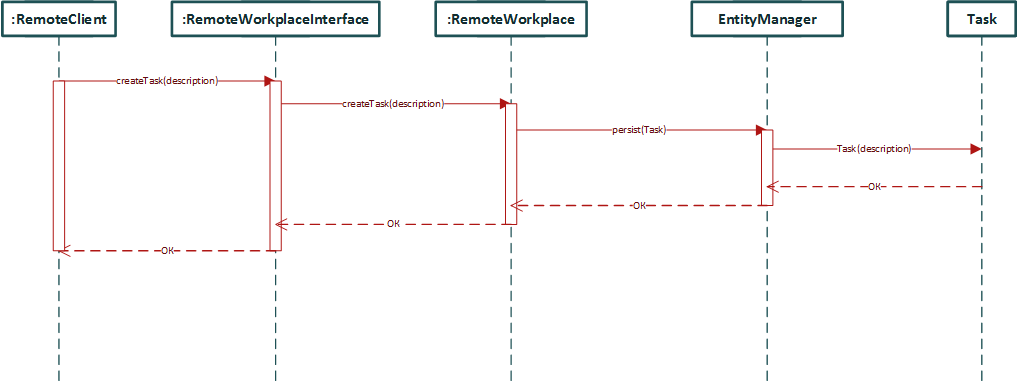
\includegraphics[width=1\textwidth]{../materials/SeqAdd.png}
	\caption{Добавление задачи}
	\label{fig:SeqAdd}
\end{figure}

\begin{figure}[H]
	\centering
	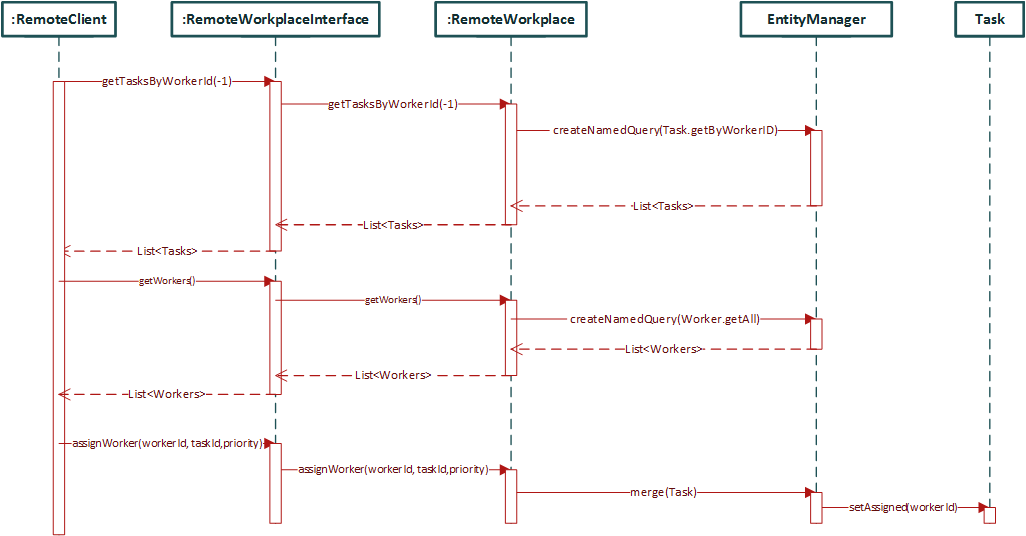
\includegraphics[width=1\textwidth]{../materials/SeqAssign.png}
	\caption{Назначение задачи}
	\label{fig:SeqAssign}
\end{figure}

\begin{figure}[H]
\centering
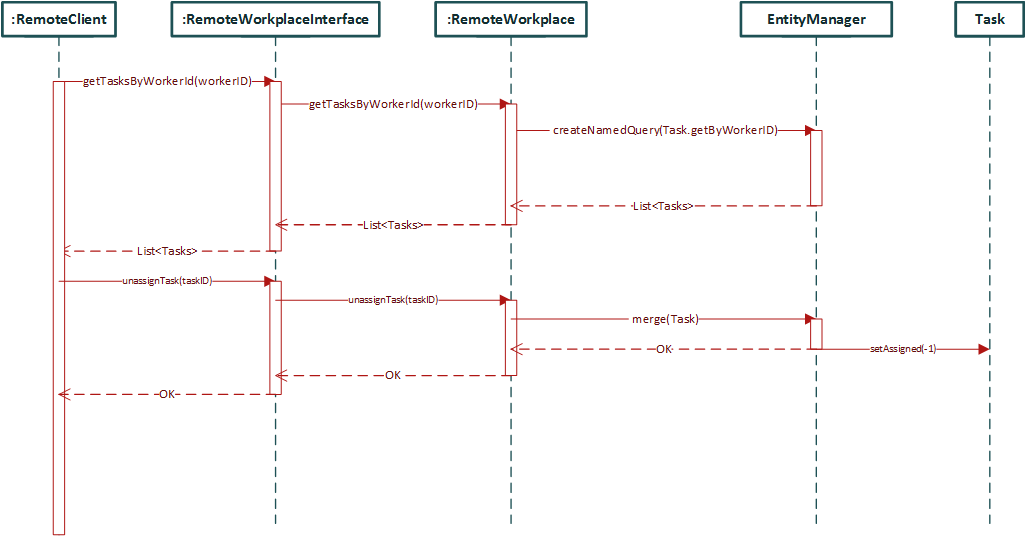
\includegraphics[width=1\textwidth]{../materials/SeqUnassign.png}
\caption{Снятие задачи}
\label{fig:SeqUnassign}
\end{figure}

\begin{figure}[H]
	\centering
	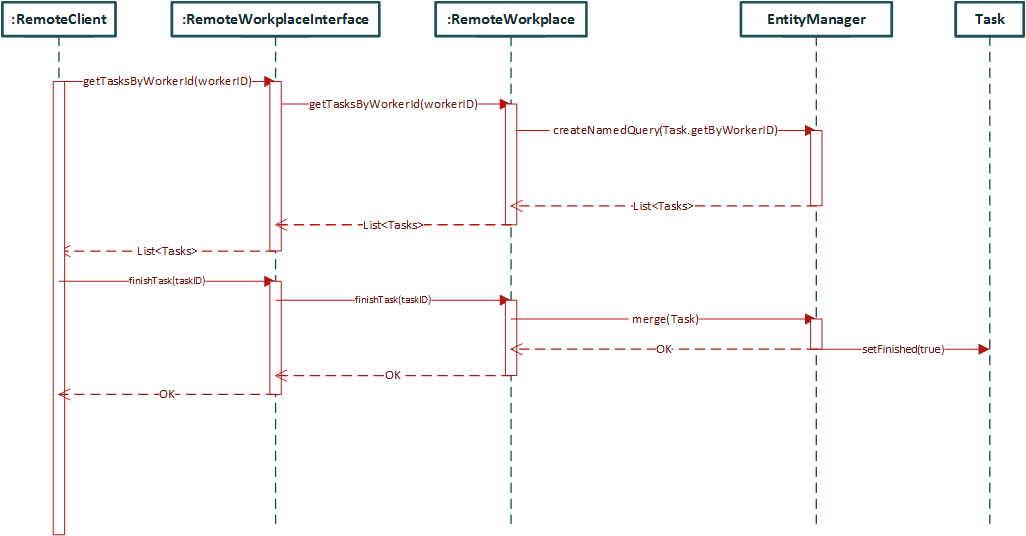
\includegraphics[width=1\textwidth]{../materials/SeqFinish.png}
	\caption{Завершение задачи}
	\label{fig:SeqFin}
\end{figure}

\begin{figure}[H]
	\centering
	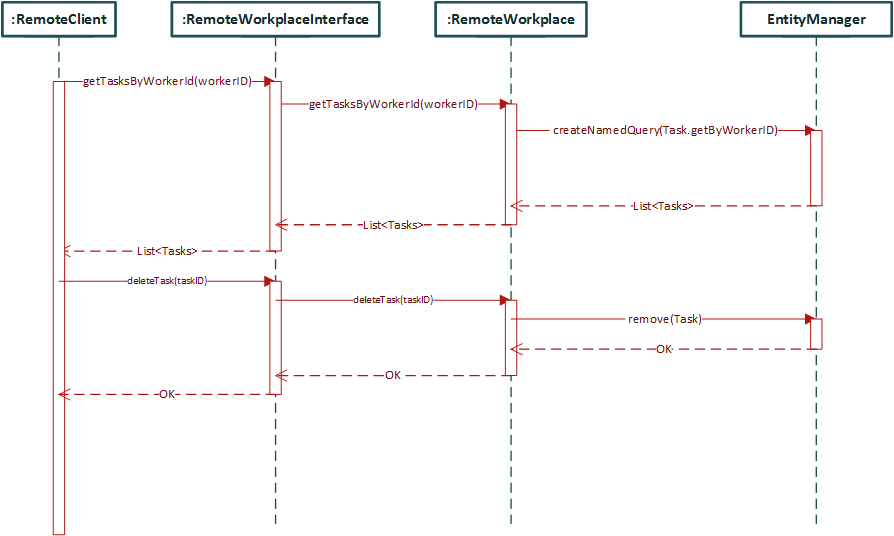
\includegraphics[width=1\textwidth]{../materials/SeqDel.png}
	\caption{Удаление задачи}
	\label{fig:SeqDel}
\end{figure}
